%\include{beamerpreamble}
\documentclass{beamer}
\usetheme{Boadilla}
\usecolortheme{wolverine}

\usepackage[T1,T2A]{fontenc}
\usepackage[utf8]{inputenc}
\usepackage[english,russian]{babel}	% Localization

\usepackage{amsmath,euscript,mathrsfs}
\usepackage{amssymb,amsfonts,latexsym,mathtools}
\usefonttheme[onlymath]{serif}
\usepackage{graphicx} 
\usepackage{wrapfig}
\usepackage{xcolor}

\usepackage{caption,tabularx}

% Absolute value declaration
\DeclarePairedDelimiter{\abs}{\lvert}{\rvert}
\DeclarePairedDelimiter{\norm}{\|}{\|}
\DeclareMathOperator{\erf}{erf}
\DeclareMathOperator{\trace}{tr}
%\DeclareMathOperator{\tg}{tg}
%\DeclareMathOperator{\ctg}{ctg}
\DeclareMathOperator{\sech}{sech}

% Page breaking in multi-line formulae
\allowdisplaybreaks[1]

% Delimiters
\newcommand{\lb}{\left (}
\newcommand{\rb}{\right )}
\newcommand{\lset}{\left \{}
\newcommand{\rset}{\right \}}
\newcommand{\lsq}{\left [}
\newcommand{\rsq}{\right ]}

% Tensors
\newcommand{\vect}[1]{\underline{#1}}
\newcommand{\tens}[1]{\underline{\underline{#1}}}

% Additional commands
\newcommand{\divg}{\text{div}}

% Big 'O' notation
\renewcommand{\O}[1]{O \lb #1 \rb}

% Equation specific commands
\newcommand{\eqtext}[1]{\quad \text{#1} \quad}
\newcommand{\RA}{\quad \Rightarrow \quad}

% Derivatives (normal and partial)
\newcommand{\dd}[1]{\; \mathrm{d} #1}
\newcommand{\diff}[2]{\frac{\mathrm{d} #1}{\mathrm{d} #2}}
\newcommand{\diffn}[3]{\dfrac{\mathrm{d}^{#1} #2}{\mathrm{d} #3^{#1}}}
\newcommand{\pdd}[1]{\; \partial #1}
\newcommand{\pdiff}[2]{\frac{\partial #1}{\partial #2}}
\newcommand{\pdiffn}[3]{\dfrac{\partial^{#1} #2}{\partial #3^{#1}}}

\setlength{\abovedisplayskip}{0pt}
\setlength{\belowdisplayskip}{1pt}


\title[Волны в нелинейно упругих телах]{Продольные волны деформации в нелинейно упругих волноводах}
\author[Ф.\,Е. Гарбузов]{Ф.\,Е. Гарбузов}
%\date{Days on Diffraction 2018}
%\institute[]{Ioffe Institute}

\begin{document}

%\frame[plain]{\titlepage}

\begin{frame}[plain]
\centering
{\footnotesize
Санкт-Петербургский политехнический университет Петра Великого\\
Институт прикладной математики и механики
}

\vspace{12mm}
Выпускная квалификационная работа магистра
\vspace{3mm}

{\Large\color{blue}
Продольные волны деформации в нелинейно упругих волноводах
}
\vspace{12mm}

{ \footnotesize 
\begin{tabularx}{.9\linewidth}{Xr}
	Выполнил студент гр. 23641/1 & Ф.\,E.~Гарбузов  
	\vspace{2mm}\\
	Руководитель (СПб\,ПУ) & Б.\,С.~Григорьев
	\vspace{2mm}\\
	Научный консультант (ФТИ им. Иоффе)  & Я.\,М.~Бельтюков
\end{tabularx} 
}
\end{frame}
 
\begin{frame}
\frametitle{Постановка задачи}
\begin{itemize}
	\item Построить асимптотическую одномерную модель для продольных волн в нелинейно упругом стержне, учитывающую нагрузку на поверхности стержня.
	\item Найти солитонные решения и проанализировать свойства выведенной модели.
	\item [Провести...] В численном моделировании сравнить полученную модель с полной трёхмерной моделью.
\end{itemize}
\end{frame}


\begin{frame} \frametitle{Полные трёхмерные уравнения}
\begin{wrapfigure}[4]{r}{125pt}
	\vspace{-2mm}
	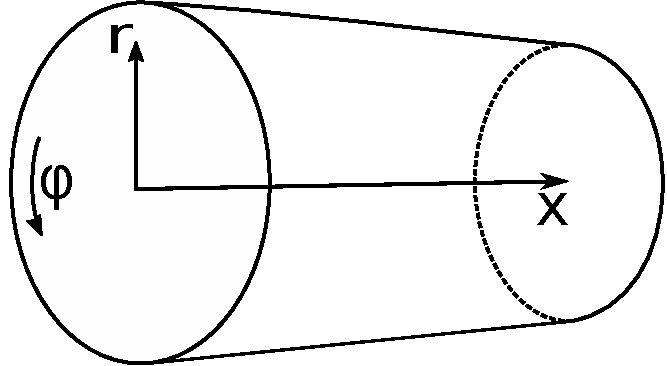
\includegraphics[width=\linewidth]{figures/1_RodSchematic}
\end{wrapfigure}
Трёхмерный вектор перемещения $\color{darkblue}\vect{U}$.\\
\vspace{1mm}
Слабонелинейная деформация (малой, но не бесконечно малой амплитуды).\\
\vspace{1mm}
Тензор деформации и плотность потенциальной энергии:
\small
\begin{align*}
%&\color{darkblue}\vect{U} - \mbox{\color{black}трёхмерный вектор перемещения}\\
&\tens{E} = \frac12 \lb(\nabla\vect{U})^T + \nabla\vect{U} + {\color{darkblue}(\nabla\vect{U})^T\cdot\nabla\vect{U}}\rb\\
&W = \frac{\lambda + 2\mu}{2}I_1(\tens{E})^2 - 2\mu I_2(\tens{E}) +\color{darkblue} \frac{l+2m}{3}I_1(\tens{E})^3 - 2m I_1(\tens{E}) I_2(\tens{E}) + n I_3(\tens{E})
%&\tens{P} = {\color{black}\lambda} \lb\trace{\tens{E}}\rb \tens{{I}} + 2{\color{black}\mu} \tens{E}\\
%&\hspace{7mm}\color{darkblue} + l \lb\trace{\tens{E}}\rb^2 \tens{{I}} - m\lb \lb\trace{\tens{E}}\rb^2\tens{{I}} - 2\lb\trace{\tens{E}}\rb\tens{E} - \lb\trace{\tens{E}^2}\rb\tens{{I}}\rb + n\lb\tens{E}^*\rb^T,
\end{align*}
$\lambda,\ \mu$ --- модули упругости Ламе (линейные),\\
$\color{darkblue}l,\ m,\ n$ --- модули упругости Мурнагана (нелинейные).\\
\vspace{1mm}
\normalsize
Полные трёхмерные уравнения движения:
\begin{equation}\nonumber
\color{darkblue}
\rho\ddot{\vect{U}} = \divg\tens{P}, \qquad \tens{P} = (\tens{I} + \nabla\vect{U}) \cdot \pdiff{W}{\tens{E}}
\end{equation}
%Уравнения дополняются граничными условиями.
\end{frame}


\begin{frame} \frametitle{Упрощающие предположения}
\begin{wrapfigure}[4]{r}{125pt}
	\vspace{-2mm}
	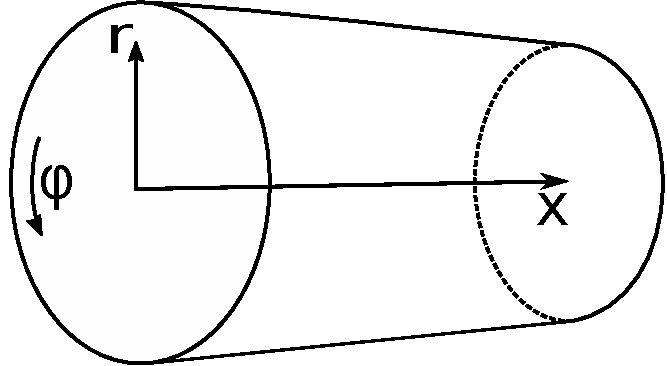
\includegraphics[width=\linewidth]{figures/1_RodSchematic}\\
	\footnotesize
	Радиус стержня --- $R$.\\
	Перемещения:\\
	$U$ --- осевое (продольное), \\
	$V$ --- радиальное (поперечное).
\end{wrapfigure}
Предположения:
\begin{itemize}
	\item Стержень бесконечен вдоль оси $x$.
	\item Осесимметричная задача: нет кручения и от угловой координаты $\varphi$ ничего не зависит.
	\item Малые деформации: $\color{darkblue}U,\ V \sim \varepsilon \ll 1$
	\item Функции медленно меняются: $\color{darkblue}\partial/\partial x,\ \partial/\partial r \sim 1/L$.
	\item Тонкий стержень: $\color{darkblue}R/L = \delta \ll 1$.
\end{itemize}
%На боковой поверхности заданы напряжения $\vect{P_b} = (P(x,t), T(x,t), 0)$.
\vspace{1mm}
Разложение перемещений в степенной ряд по радиальной переменной:
%\color{darkblue}
\begin{align*}
U(x,r,t) &= U_0(x,t) + r^2 U_2(x,t) + r^4 U_4(x,t) + \dots \, ,\\
V(x,r,t) &= r V_1(x,t) + r^3 V_3(x,t) + r^5 V_5(x,t) + \dots \, .
\end{align*}
Подстановка разложений в уравнения движения позволяет выразить $U_2,\ V_3,\ U_4,\ V_5$ через $U_0$ и $V_1$. 
\end{frame}


\begin{frame} \frametitle{Упрощённая система двух уравнений}
На границе задано нормальное напряжение $P(x,t)$ и касательное $T(x,t)$:
\small
\begin{align*} \nonumber
\begin{split}
&2 (\lambda + \mu) {\color{red}V_1} + \lambda {\color{darkblue}U_{0x}} +\varepsilon \Psi_1({\color{darkblue}U_{0}}, {\color{red}V_1}) + \delta^2 \bigg[ \gamma_1 {\color{darkblue}U_{0xxx}} + \gamma_2 {\color{darkblue}U_{0xtt}} + \gamma_3 {\color{red}V_{1tt}} + \gamma_4 {\color{red}V_{1xx}}\bigg] +\\
&\hspace{70mm}+ O(\varepsilon^2, \varepsilon\delta^2, \delta^4) =  \frac{\mu(3\lambda + 2\mu)}{\lambda + \mu} P,
\end{split}\\
\begin{split}
&\rho  c^2 {\color{darkblue}U_{0tt}} -2 \lambda {\color{red}V_{1x}}-(\lambda +2 \mu ) {\color{darkblue}U_{0xx}} - \varepsilon \Psi_2({\color{darkblue}U_{0}}, {\color{red}V_1})
+ \delta^2\bigg[\gamma_5 {\color{darkblue}U_{0xxxx}} + \gamma_6 {\color{darkblue}U_{0tttt}} + \\
&\hspace{18mm}+ \gamma_7 {\color{darkblue}U_{0xxtt}} + \gamma_8 {\color{red}V_{1xxx}} + \gamma_9 {\color{red}V_{1xtt}} \bigg] + O(\varepsilon^2, \varepsilon\delta^2, \delta^4) = \frac{2\mu(3\lambda + 2\mu)}{\lambda + \mu} T.
\end{split}
\end{align*}
Коэффициенты $\gamma_j$ зависят от упругих модулей, $\Psi$ --- нелинейные функции.\\
\vspace{1mm}
\normalsize
Существует два способа исключения ${\color{red}V_1}$, приводящие к одномерному уранению типа Буссинеска.
\end{frame}


\begin{frame} \frametitle{Уравнения типа Буссинеска}
$u = U_{0x}$ --- продольная деформация, $c = \sqrt{E/\rho}$ --- скорость длинных линейных волн.
\small
\begin{align*}
&u_{tt} - c^2 u_{xx} - \frac{2}{\rho}\bigg(\nu P_{xx} + \frac1R T_x\bigg) - {\color{darkblue}\left(\frac{\beta_1}{2\rho} u^2 + \frac{\beta_2}{\rho E} u P + \frac{\beta_3}{2\rho E^2} P^2\right)_{xx}} +\\
&\hspace{10mm} + {\color{red}R^2 \bigg(\frac{\alpha_1^{(i)}}{c^2} u_{tttt} + \alpha_2^{(i)} u_{xxtt} + c^2\alpha_3^{(i)} u_{xxxx} + G^{(i)}(P, T) \bigg)} = 0, \quad i = 1,2.\\
&\color{black}\mbox{\color{black}\normalsize Солитонное решение: } u_i(x,t) = A\ {\rm sech}^2\ \left[B_{i} \left(x\pm t \sqrt{c^2+\frac{A \beta_1}{3 \rho}}\right) \right].&
%&B_i = \sqrt{\frac{3A\beta_1 E}{-4\left[(A\beta_1 + 3E)^2\alpha_1^{(i)} + 3E(A\beta_1 + 3E)\alpha_2^{(i)} + 9E^2\alpha_3^{(i)}\right] R^2}} \, , \quad i = \overline {1,4}.
\end{align*}
\begin{figure}
	\vspace{-6mm}
	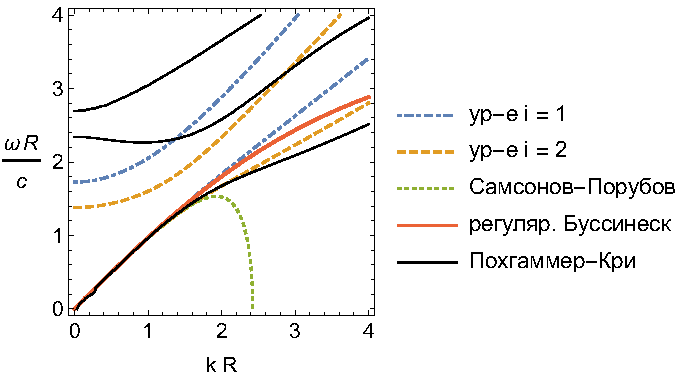
\includegraphics[width=.6\linewidth]{figures/DispColorSmall}
	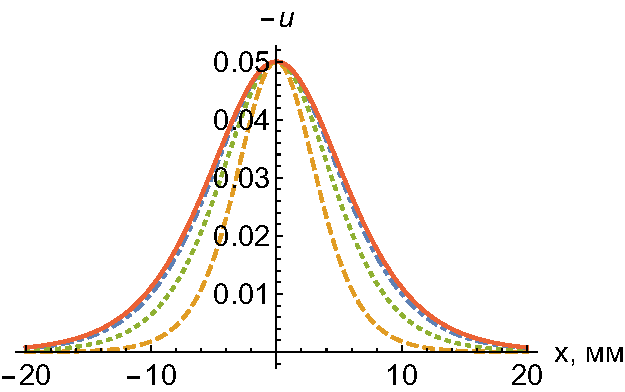
\includegraphics[width=.39\linewidth]{figures/FourSolitonsColor2}
	%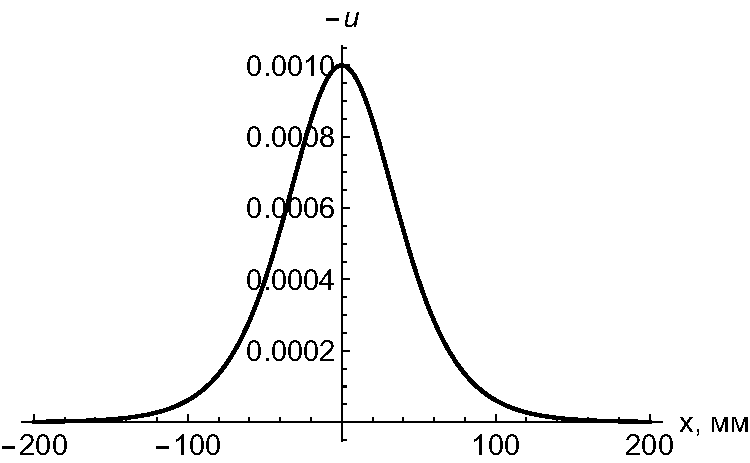
\includegraphics[width=.44\linewidth]{figures/3b_SingleSoliton}
\end{figure}

\end{frame}


\begin{frame} \frametitle{Численная схема}
\begin{figure}[h!]
	\centering
	%\begin{subfigure}{0.5\textwidth}
	\centering
	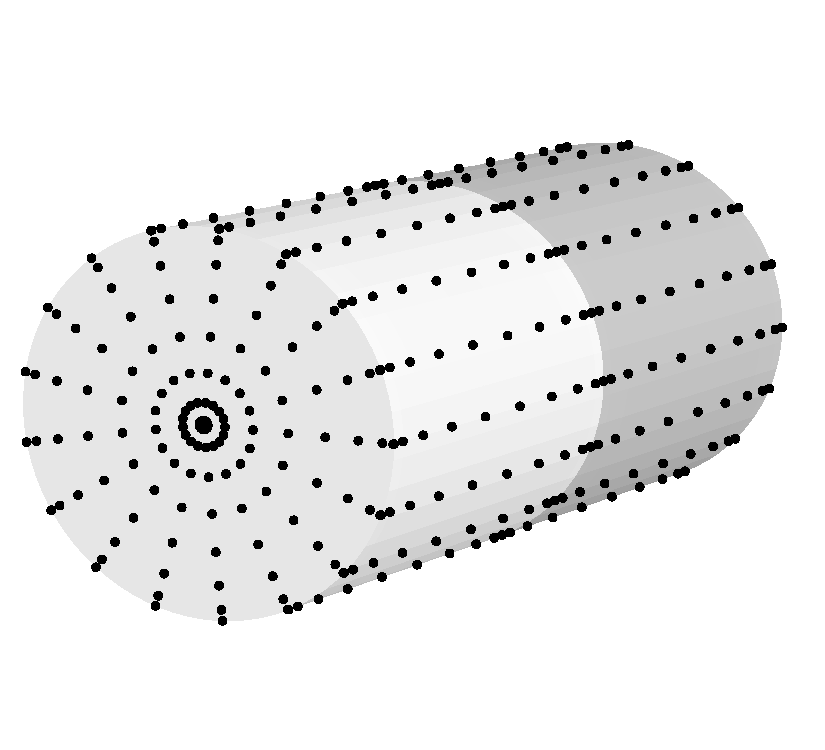
\includegraphics[width=.35\textwidth]{figures/Grid3D}
	%\caption{Lorem ipsum}
	%\end{subfigure}
	%\begin{subfigure}{0.48\textwidth}
	%		\centering
	%		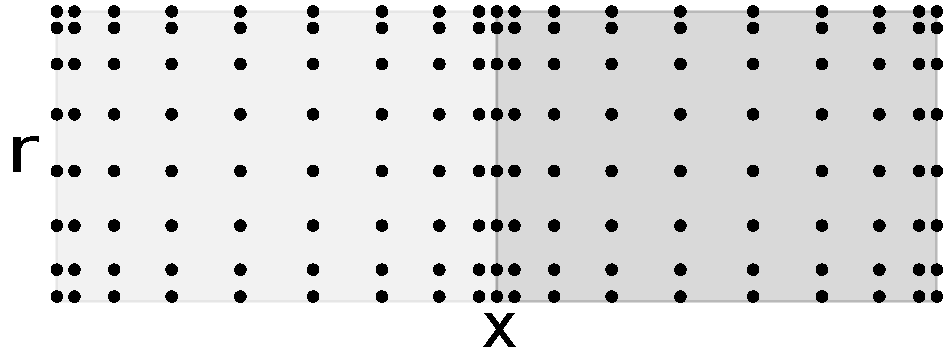
\includegraphics[width=\textwidth]{figures/Grid2D}
	%\caption{Lorem ipsum}
	%	\end{subfigure}
	\caption{Cетка из двух доменов.}
\end{figure}
\end{frame}


\begin{frame} \frametitle{Сравнение моделей: эволюция волны}
\begin{figure}[h]
	\centering
	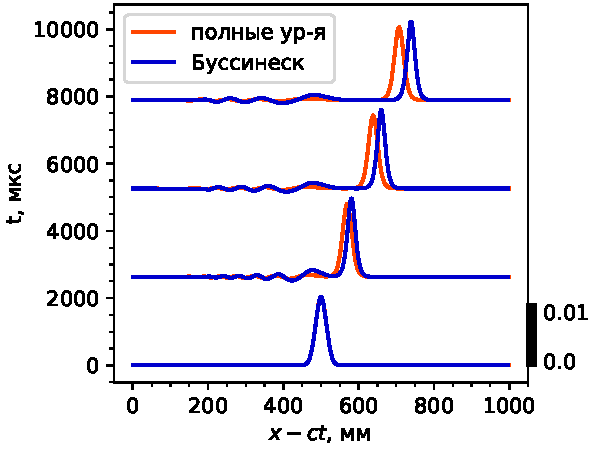
\includegraphics[width=0.49\linewidth]{figures/SolEvolCompareSmallColor}
	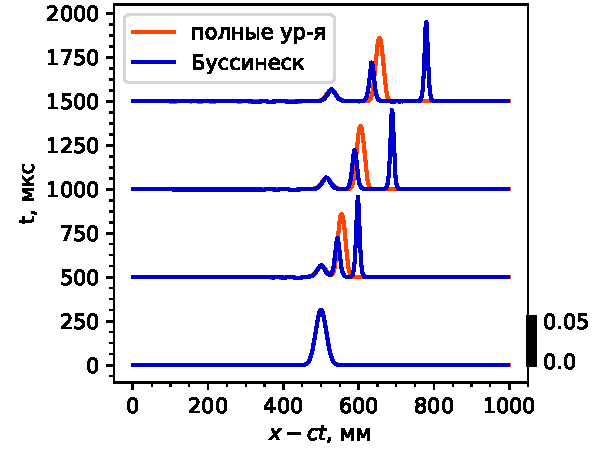
\includegraphics[width=0.49\linewidth]{figures/SolEvolCompareSmallColor2}
	\caption{Профили решений $-u(x-ct, t)$ регуляризованного уравнения Буссинеска и продольной деформации $-U_x(x - ct, 0, t)$ в центре стержня ($r=0$) в различные моменты времени. Масштаб амплитуды деформации показан чёрным прямоугольником.}
\end{figure}
\end{frame}


\begin{frame} \frametitle{Сравнение моделей: скорость-амплитуда}
%Начальные условия:
%\begin{align*}
%& U_0 (x, r) = A_0 W \erf\lb \frac{x - L/2}{W}\rb,&  &\dot{U}_0 (x, r) = -c \pdiff{U_0}{x}\\
%& V_0(x, r) = -\nu r \pdiff{U_0}{x},& &\dot{V}_0 (x, r) = -c \pdiff{V_0}{x}
%\end{align*}
\begin{wrapfigure}[10]{r}{200pt}
	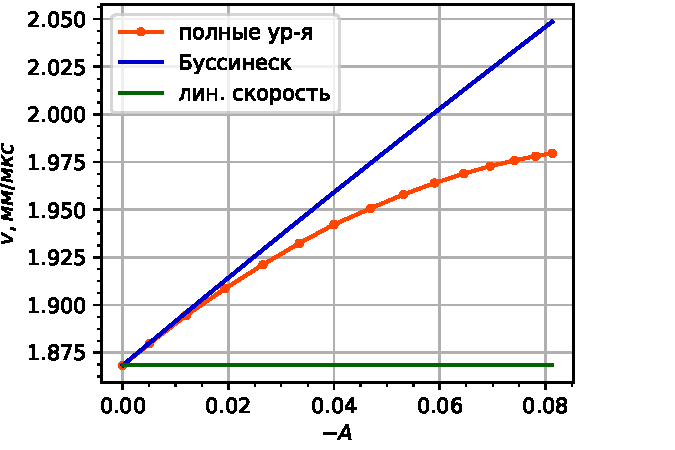
\includegraphics[width=\linewidth]{figures/VelAmplColor}
	%\caption{Зависимость скорости солитона от амплитуды. Горизонтальная линия --- скорость линейных волн $c$.}
\end{wrapfigure}
Зависимость скорости от амплитуды в модели Буссинеска:
\begin{equation}\nonumber
v(A) = \sqrt{c^2 + A\frac{\beta_1}{3\rho}}
\end{equation}
Зависимость для полных уравнений получена в серии численных экспериментов.
\end{frame}


\begin{frame} \frametitle{Сравнение моделей: удар по поверхности}
\begin{figure}[h]
	\centering
	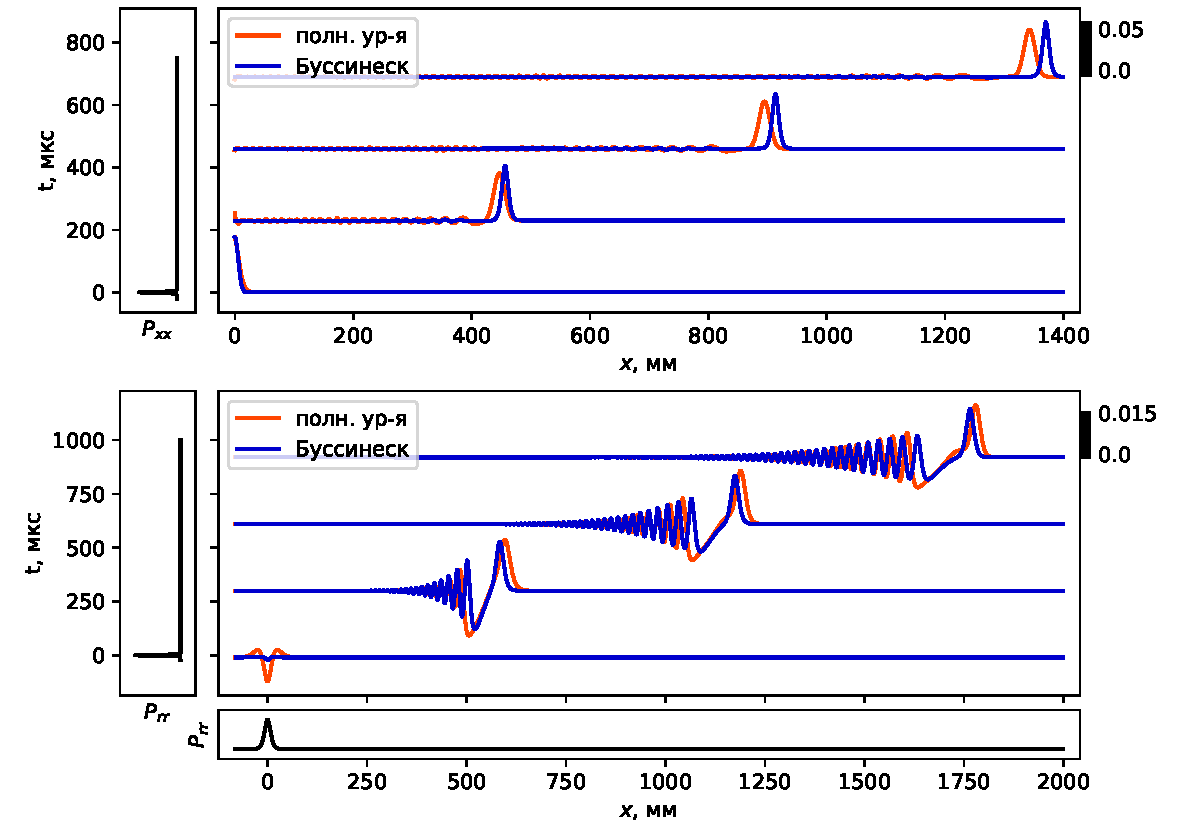
\includegraphics[width=.93\linewidth]{figures/Impact2Color}
\end{figure}
\end{frame}


\begin{frame} \frametitle{Заключение}
%Результаты:
\begin{itemize}
	\item Выведены две новые асимптотические модели типа Буссинеска с внешним воздействием, описывающие продольные волны в нелинейно упругих стержнях круглого сечения.
	\item Построен метод, позволяющий численно моделировать полные трёхмерные уравнения движения стержня в рамках нелинейной теории упругости.
	\item Численно решён ряд начально-краевых задач, показывающих хорошую применимость уравнения типа Буссинеска для моделирования возникновения солитонов деформации.
\end{itemize}
%Для описания продольных длинных волн в стержнях круглого сечения мы вывели две новые асимптотические модели типа Буссинеска, отличающиеся друг от друга коэффициентами при дисперсионных слагаемых. Эти модели обобщены на случай ненулевой осесимметричной нагрузки на боковой поверхности, а также на случай предварительно растянутого стержня.

%Нам удалось построить метод, позволяющий численно моделировать полные трёхмерные уравнения движения стержня в рамках нелинейной теории упругости. Мы численно решили ряд начально-краевых задач и показали хорошую применимость модели типа Буссинеска для моделирования возникновения солитонов.

Статьи и конференции:
\footnotesize
\begin{enumerate}
	\item Garbuzov F.\,E., Khusnutdinova K.\,R., Semenova I.\,V., On Boussinesq-type models for long longitudinal waves in elastic rods, \textit{Wave Motion} 88 (2019) 129--143.
	\item International Conference ''Days on Diffraction 2018'', Steklov Mathematical Institute, St.  Petersburg, Russia, 4 - 8 June 2018, oral presentation.
\end{enumerate}

\end{frame}

\end{document}